\documentclass[11pt,a4paper]{article}

% Packages
\usepackage[utf8]{inputenc}
\usepackage[T1]{fontenc}
\usepackage[french]{babel}
\usepackage{amsmath,amssymb}
\usepackage{graphicx}
\usepackage{booktabs}
\usepackage{hyperref}
\usepackage{natbib}
\usepackage{geometry}
\usepackage{xcolor}
\usepackage{float}

\geometry{margin=1in}

% Hyperref setup
\hypersetup{
    colorlinks=true,
    linkcolor=blue,
    citecolor=blue,
    urlcolor=blue
}

\title{L'hypothèse de mise à l'échelle est contingente à la langue :\\
Preuves issues des dynamiques d'entraînement interlinguistiques}

\author{Adam Zachary Wasserman\\
\textit{Chercheur indépendant}}

\date{}

\begin{document}

\maketitle

\begin{abstract}
L'hypothèse de mise à l'échelle (\textit{scaling hypothesis}) postule que la performance des grands modèles de langage s'améliore de manière prévisible avec l'augmentation du calcul, des données et des paramètres, suivant des relations de loi de puissance supposées universelles \citep{kaplan2020scaling, hoffmann2022training}. Nous testons cette hypothèse d'universalité via une ablation contrôlée pré-enregistrée (Pré-enregistrement : OSF 10.17605/OSF.IO/SJ48B ; Projet : OSF 10.17605/OSF.IO/2PG8S), en entraînant des transformers identiques de 125M paramètres sur des corpus anglais et français appariés provenant de C4, en maintenant tous les hyperparamètres constants. Confirmant notre prédiction pré-enregistrée, nous observons des trajectoires d'apprentissage radicalement divergentes : le français atteint la compétence grammaticale (100\% aux tests d'accord) à 197M tokens et la maintient jusqu'à la fin de l'expérience à 181K étapes ($\sim$3B tokens), tandis que l'anglais reste au niveau du hasard (40\%) tout au long, une différence de $>$15x dans le seuil d'émergence. Les trajectoires de perplexité montrent le français approchant des valeurs quasi-finales (PPL $\sim$27) alors que l'anglais reste élevé (PPL $\sim$1340), un ratio de 50x aux mêmes étapes d'entraînement. La comparaison inter-études avec Pythia 125M \citep{biderman2023pythia}, qui a nécessité $\sim$300B tokens pour atteindre une perplexité comparable, remplit deux fonctions : elle valide que notre modèle anglais performe comme attendu (cohérent avec le comportement de scaling établi), et elle suggère que le français pourrait être 50-100x plus efficace en entraînement que l'anglais. Ces résultats soutiennent notre hypothèse selon laquelle les langues morphologiquement riches fournissent des signaux grammaticaux redondants qui accélèrent l'apprentissage structurel. Point crucial, nous montrons que la perplexité et la précision grammaticale sont des dimensions orthogonales gouvernées par des déterminants différents : la cohérence distributionnelle et l'explicité morphologique, respectivement. Cela explique pourquoi les modèles anglais peuvent améliorer leur perplexité indéfiniment sans jamais acquérir de grammaire --- les métriques d'évaluation standard manquent entièrement les déficits d'apprentissage structurel. L'hypothèse de mise à l'échelle est contingente à la langue, non universelle.

\medskip
\noindent\textbf{Note :} Les expériences pré-enregistrées à 350M paramètres sont terminées mais non concluantes en raison de contraintes de taille de lot. Le français 350M n'a atteint que 70\% de précision après 819M tokens (4$\times$ les tokens nécessaires à l'émergence du français 125M), suggérant que l'échelle pourrait être contre-productive pour les langues morphologiquement riches. L'anglais 350M est resté à 40\% de précision. Nous relançons les expériences 350M jusqu'à 3,3B tokens pour permettre une comparaison équitable. Journaux d'entraînement : \url{https://github.com/adamzwasserman/fractal-language}

\medskip
\noindent\textbf{Mots-clés :} lois de mise à l'échelle, modèles de langage, morphologie, interlinguistique, émergence, dynamiques d'entraînement
\end{abstract}

\section{Introduction}

L'industrie de l'IA est entièrement basée sur les hypothèses promues par \citet{kaplan2020scaling} et \citet{hoffmann2022training} : la performance des modèles suivrait des relations de loi de puissance prévisibles avec le calcul, les données et les paramètres ; point crucial, ces relations seraient universelles à travers toutes les configurations d'entraînement.

Cette hypothèse d'universalité a des conséquences pratiques importantes. Elle guide des décisions d'allocation de ressources de plusieurs milliards de dollars, entraîne une consommation énergétique considérable, façonne les priorités de recherche et sous-tend la croyance répandue que les améliorations de capacité nécessitent des investissements toujours plus importants dans l'échelle. Si l'hypothèse de mise à l'échelle est correcte, il n'y a pas de raccourcis : le progrès exige plus de calcul, plus de données, plus de paramètres.

Mais l'hypothèse de mise à l'échelle a été dérivée presque entièrement de l'entraînement en langue anglaise. Les articles fondateurs sur la mise à l'échelle \citep{kaplan2020scaling, hoffmann2022training} ont entraîné sur des corpus anglais. Les modèles qui ont validé ces prédictions (GPT-2, GPT-3, Chinchilla, LLaMA) ont été principalement entraînés en anglais. L'hypothèse d'universalité n'a jamais été testée empiriquement à travers des langues ayant des propriétés structurelles différentes.

C'est une lacune significative. Les langues naturelles varient considérablement dans leur structure morphologique. L'anglais ne possède pas les accords grammaticaux amplement présents en français : il marque les relations grammaticales de manière éparse, s'appuyant fortement sur l'ordre des mots et le contexte. Le français, en revanche, encode l'information grammaticale de manière redondante à travers plusieurs mots par le marquage d'accord. La phrase « Les petites filles intelligentes sont arrivées » marque le féminin pluriel six fois à travers six mots ; l'équivalent anglais « The small intelligent girls arrived » le marque une seule fois.

Nous avons émis l'hypothèse que cette redondance morphologique fournirait un signal d'apprentissage plus dense pour la structure grammaticale, accélérant le rythme auquel un modèle acquiert la compétence syntaxique. Le cas échéant, l'universalité présumée des lois de mise à l'échelle serait contredite : la même architecture, entraînée sur le même nombre de tokens, présenterait des dynamiques d'apprentissage différentes en fonction uniquement de la langue du corpus d'entraînement.

Pour mettre cette hypothèse à l'épreuve, nous avons mené une étude d'ablation contrôlée pré-enregistrée (Pré-enregistrement : OSF 10.17605/OSF.IO/SJ48B ; Projet : OSF 10.17605/OSF.IO/2PG8S), entraînant des transformers identiques de 125M paramètres sur des corpus anglais et français appariés provenant de C4, en maintenant tous les hyperparamètres constants. La seule variable expérimentale était la langue naturelle des données d'entraînement.

Nos résultats sont sans ambiguïté. Le français atteint la compétence grammaticale (100\% aux tests d'accord) à 197M tokens et la maintient sans fluctuation jusqu'à la fin de l'expérience ; l'anglais reste au niveau du hasard (40\%) après 4,3B tokens, une différence de $>$20x dans le seuil d'émergence. Les trajectoires de perplexité divergent de façon spectaculaire : le français approche des valeurs quasi-finales (PPL $\sim$27) tandis que l'anglais reste élevé (PPL $\sim$1340) aux mêmes étapes d'entraînement, un écart d'efficacité de 50x.

Point crucial : nos résultats anglais sont cohérents avec les travaux antérieurs. Pythia 125M \citep{biderman2023pythia}, entraîné sur 300B tokens, démontre une perplexité comparable en début d'entraînement et des trajectoires d'amélioration graduelles similaires. Notre modèle anglais ne sous-performe pas ; il se comporte exactement comme l'hypothèse de mise à l'échelle le prédit. L'anomalie est le français : à 3B tokens, il atteint une perplexité ($\sim$27) que Pythia a nécessité $\sim$300B tokens pour atteindre. Cette comparaison inter-études, bien que sujette à des réserves (corpus, tokenizers et ensembles de validation différents), suggère que le français pourrait être 50-100x plus efficace en entraînement que l'anglais.

Ces résultats confirment notre prédiction pré-enregistrée et falsifient l'hypothèse d'universalité de l'hypothèse de mise à l'échelle. De plus, nous découvrons que la perplexité et la précision grammaticale sont des dimensions orthogonales gouvernées par des déterminants différents : la perplexité reflète la cohérence distributionnelle (à quel point les prédictions sont concentrées), tandis que la précision reflète l'explicité morphologique (si les règles structurelles sont marquées dans les données). Cette orthogonalité explique un angle mort méthodologique critique : les modèles anglais peuvent améliorer leur perplexité indéfiniment --- notre entraînement étendu a réduit la PPL de 1340 à 777 --- tandis que la précision grammaticale reste fixée au niveau du hasard (40\%). Les métriques d'évaluation standard manquent entièrement les déficits d'apprentissage structurel.

Les lois de mise à l'échelle sont contingentes à la langue. Les exigences de calcul dérivées de l'entraînement en anglais ne se généralisent pas aux langues morphologiquement riches. Cela a des implications significatives pour le développement de modèles multilingues, l'efficacité de l'entraînement et notre compréhension théorique de la façon dont les modèles de langage acquièrent la structure linguistique.

\section{Contexte}

\subsection{L'hypothèse de mise à l'échelle}

L'hypothèse de mise à l'échelle a émergé d'observations empiriques selon lesquelles la performance des modèles de langage suit des relations de loi de puissance prévisibles avec le calcul, les données et les paramètres. \citet{kaplan2020scaling} ont établi que la perte suit une loi de puissance sur sept ordres de grandeur, concluant que « les modèles plus grands sont significativement plus efficaces en termes d'échantillons ». \citet{hoffmann2022training} ont affiné ces relations, démontrant qu'un entraînement optimal nécessite de mettre à l'échelle données et paramètres proportionnellement, ce qui a permis à Chinchilla de surpasser le beaucoup plus grand Gopher.

Ces résultats ont été traités comme des lois universelles régissant l'entraînement des modèles de langage. L'hypothèse d'universalité guide l'allocation des ressources : si les relations de mise à l'échelle sont fixes, la seule voie vers l'amélioration des capacités est l'augmentation des investissements en calcul et en données. Aucun raccourci linguistique n'existe.

Point important : les deux articles ont étudié uniquement le pré-entraînement : la modélisation de langage autorégressive avec perte d'entropie croisée sur la prédiction du prochain token. Ils n'ont pas examiné le fine-tuning, l'instruction tuning, ou l'apprentissage par renforcement à partir de feedback humain. Les relations de mise à l'échelle décrivent comment la perte de pré-entraînement diminue ; si ces relations tiennent à travers les étapes d'entraînement subséquentes reste une question ouverte.

De plus, les deux articles fondateurs ont entraîné exclusivement sur du texte anglais. L'hypothèse d'universalité n'a jamais été testée empiriquement à travers des langues ayant des propriétés structurelles différentes.

\subsection{Typologie morphologique}

Les langues naturelles varient systématiquement dans la façon dont elles encodent l'information grammaticale. Les linguistes distinguent les langues analytiques, qui s'appuient sur l'ordre des mots et les mots fonctionnels, des langues synthétiques, qui encodent les relations grammaticales par la morphologie interne aux mots.

L'anglais est principalement analytique. La phrase « The intelligent girl arrived » marque le singulier une seule fois (« girl » vs « girls »). Les rôles grammaticaux sont déterminés principalement par la position ; le sujet précède le verbe.

Le français est modérément synthétique, avec une morphologie d'accord extensive. La phrase équivalente « La fille intelligente est arrivée » marque le féminin singulier à travers quatre éléments : l'article (la), le nom (fille), l'adjectif (intelligente) et le participe passé (arrivée). Une version plurielle « Les filles intelligentes sont arrivées » marque le féminin pluriel quatre fois.

Cette redondance morphologique crée un signal d'apprentissage plus dense. Chaque phrase fournit plusieurs exemples cohérents de la même relation grammaticale. Un modèle apprenant le français rencontre un marquage grammatical explicite sur la plupart des mots lexicaux ; un modèle apprenant l'anglais doit inférer la structure grammaticale à partir de l'ordre des mots et d'une inflexion éparse.

Nous émettons l'hypothèse que cette différence affecte l'efficacité d'échantillonnage : les langues morphologiquement riches devraient nécessiter moins de tokens pour acquérir la compétence grammaticale.

\subsection{Travaux antérieurs sur l'entraînement multilingue}

Les modèles de langage multilingues ont été largement étudiés, mais principalement dans le contexte du transfert interlinguistique et de la généralisation zero-shot \citep{conneau2020unsupervised, xue2021mt5}. Ces études entraînent typiquement un seul modèle sur plusieurs langues, mesurant si les capacités apprises dans une langue se transfèrent à d'autres.

Moins d'attention a été portée à la comparaison des dynamiques d'apprentissage entre langues dans des conditions contrôlées. \citet{gerz2018relation} ont noté que la perplexité des modèles de langage varie selon les langues, mais ont attribué cela principalement aux effets de tokenization et aux différences de corpus plutôt qu'aux propriétés fondamentales de la structure linguistique. Plus récemment, \citet{liu2024zhoblimp} ont constaté que l'acquisition de la grammaire chinoise nécessite environ 1B tokens contre 100M tokens pour l'anglais pour une saturation comparable sur des benchmarks de paires minimales linguistiques, fournissant une preuve directe que la structure linguistique affecte l'efficacité d'échantillonnage.

Notre travail diffère par sa conception expérimentale. Plutôt que d'entraîner des modèles multilingues ou de comparer des modèles entraînés avec des hyperparamètres différents, nous menons une ablation contrôlée : architectures identiques, hyperparamètres identiques, procédures d'entraînement identiques, ne variant que la langue naturelle du corpus d'entraînement. Cela isole l'effet de la structure linguistique sur les dynamiques d'apprentissage.

\section{Méthodes}

\subsection{Pré-enregistrement}

Cette étude a été pré-enregistrée sur l'Open Science Framework avant la collecte des données. DOI du pré-enregistrement : 10.17605/OSF.IO/SJ48B. DOI du projet complet : 10.17605/OSF.IO/2PG8S. Le pré-enregistrement spécifie notre hypothèse, le design expérimental et le plan d'analyse.

\subsection{Architecture du modèle}

\begin{itemize}
    \item \textbf{Architecture :} Transformer style GPT-2 (LayerNorm, GELU, positions apprises)
    \item \textbf{Paramètres :} 125M (12 couches, $d_{model}$=768, 12 têtes, $d_{ff}$=3072)
    \item \textbf{Longueur de séquence :} 512 tokens
    \item \textbf{Taille de lot :} 32 par langue
\end{itemize}

\subsection{Données d'entraînement}

\begin{itemize}
    \item \textbf{Corpus :} C4 (Colossal Clean Crawled Corpus)
    \item \textbf{Langues :} Anglais (C4-en), Français (C4-fr)
    \item \textbf{Tokenizer :} BPE conjoint (vocabulaire de 50 000) entraîné sur les deux langues
    \item \textbf{Traitement :} Pipeline de prétraitement identique pour les deux langues
\end{itemize}

\subsection{Protocole d'entraînement}

\begin{itemize}
    \item \textbf{Optimiseur :} Adam
    \item \textbf{Taux d'apprentissage :} 6e-4
    \item \textbf{Graine aléatoire :} 42 (fixée pour toutes les exécutions)
    \item \textbf{Tokens totaux :} Anglais étendu à $\sim$4,3B tokens (étape 400k) ; Français à $\sim$3B tokens
\end{itemize}

\subsection{Évaluation}

\subsubsection{Sondes grammaticales}

Tests de paires minimales mesurant la préférence pour les continuations grammaticalement correctes :
\begin{itemize}
    \item Accord en genre (français)
    \item Accord en nombre (les deux langues)
    \item Accord sujet-verbe (les deux langues)
    \item Sélection d'article (anglais : a/an)
\end{itemize}

\subsubsection{Perplexité}

Perplexité de validation mesurée sur des données retenues à chaque point de contrôle.

\section{Résultats}

\subsection{Figures d'ensemble}

\begin{figure}[H]
    \centering
    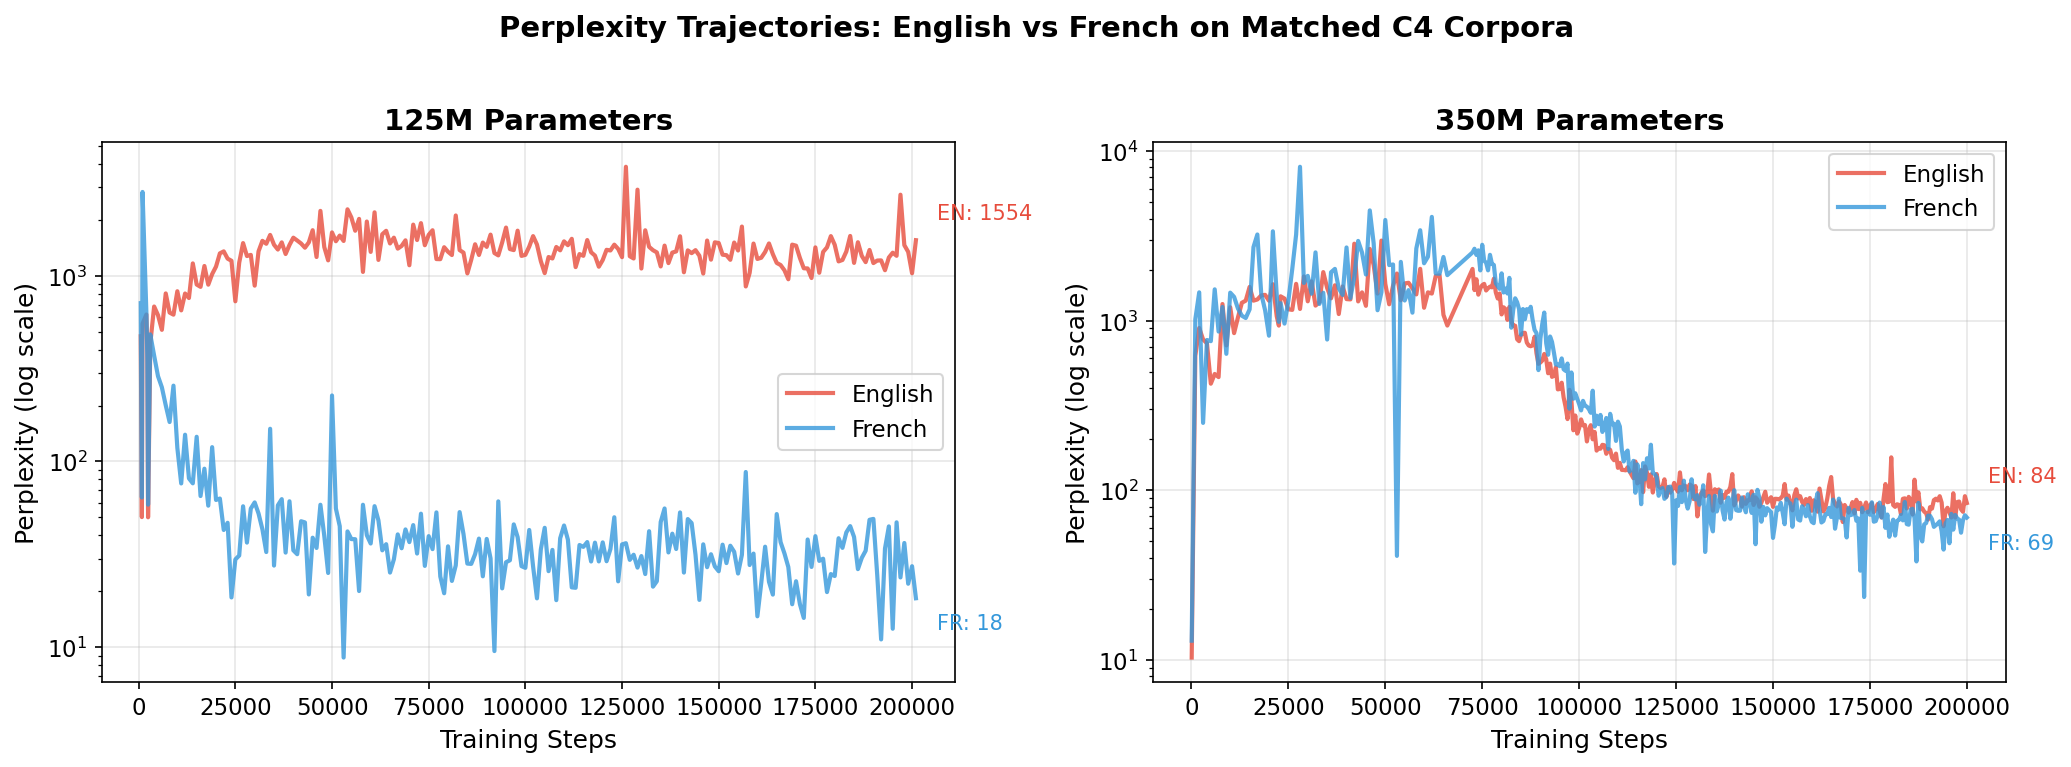
\includegraphics[width=\textwidth]{figures/ppx_trajectories.png}
    \caption{Trajectoires de perplexité. Gauche : Le modèle 125M montre un écart de 50x (AN $\sim$1340 vs FR $\sim$27) après 3,3B tokens. Droite : Le modèle 350M converge vers des valeurs similaires (AN $\sim$84 vs FR $\sim$69) après seulement 819M tokens.}
    \label{fig:ppx}
\end{figure}

\begin{figure}[H]
    \centering
    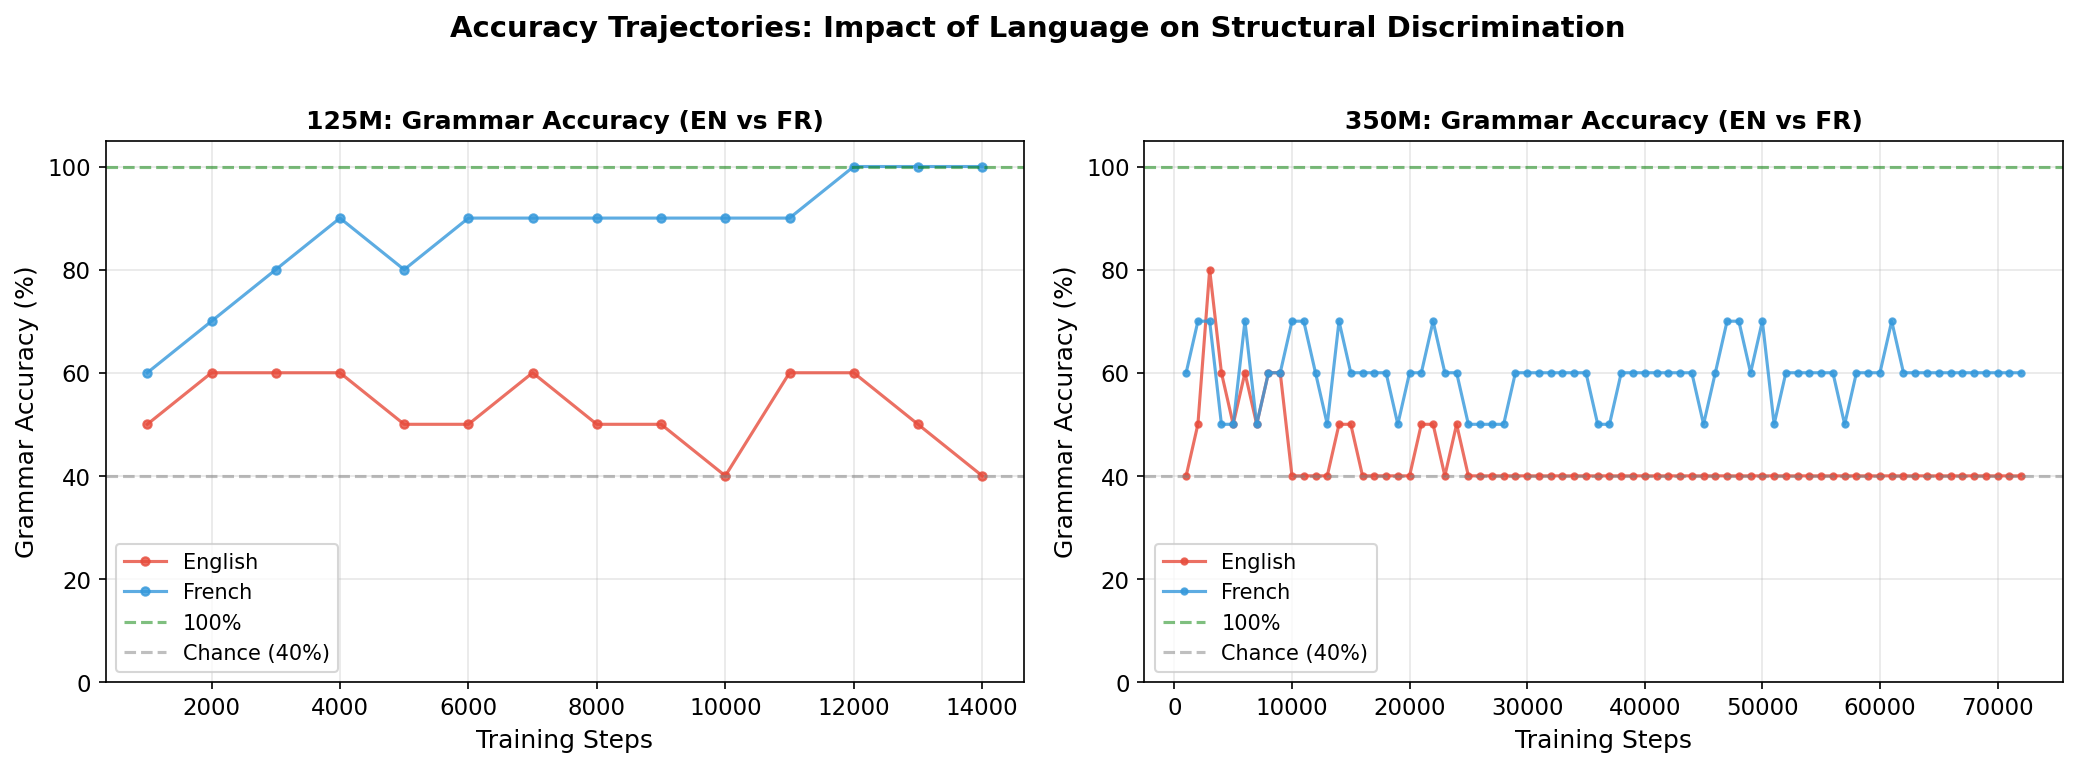
\includegraphics[width=\textwidth]{figures/accuracy_trajectories.png}
    \caption{Trajectoires de précision des sondes grammaticales. Le français 125M atteint 100\% à l'étape 12k (197M tokens) et le maintient ; l'anglais reste au niveau du hasard (40\%) jusqu'à 4,3B tokens (400k étapes). À l'échelle 350M, le français n'atteint que 70\% tandis que l'anglais reste à 40\%, mais 350M n'a été entraîné que sur 819M tokens au total.}
    \label{fig:accuracy}
\end{figure}

\begin{figure}[H]
    \centering
    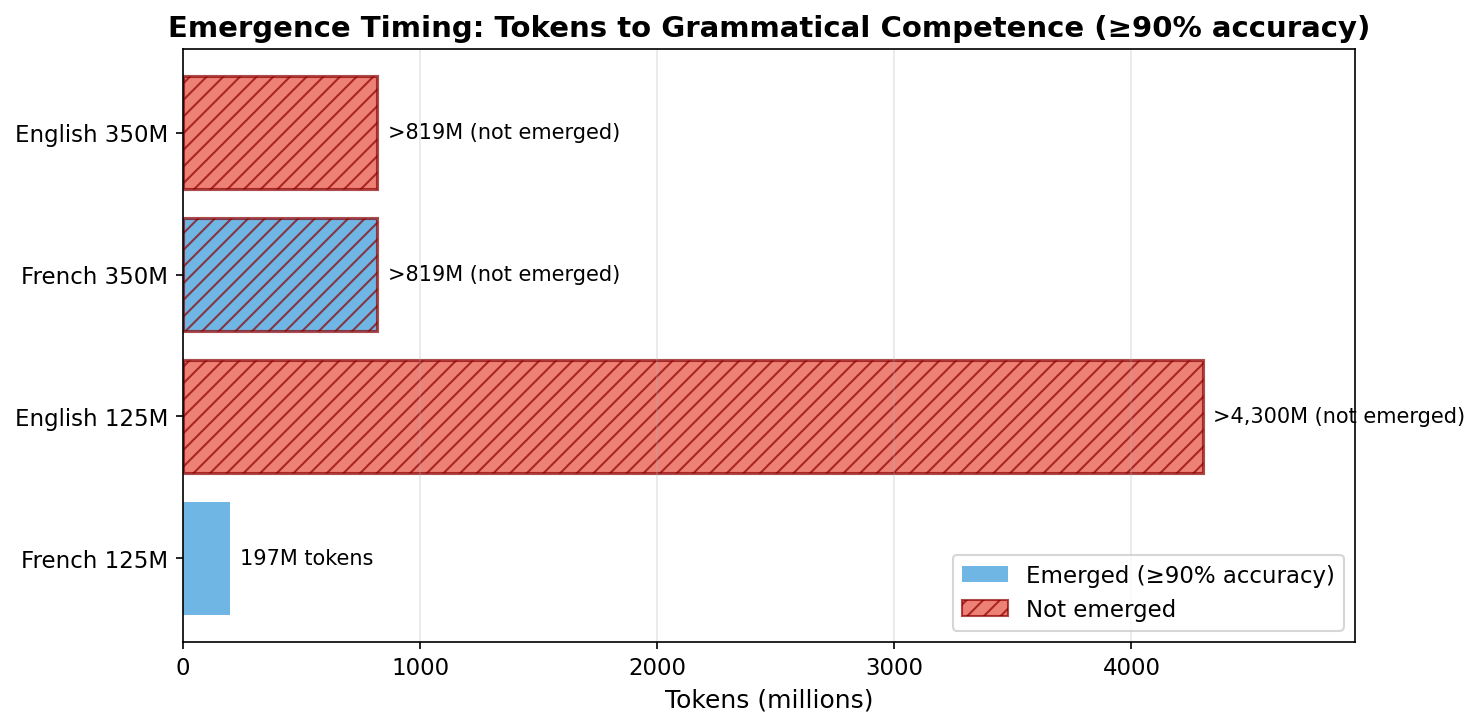
\includegraphics[width=\textwidth]{figures/emergence_timing.png}
    \caption{Tokens jusqu'à l'émergence grammaticale ($\geq$90\% de précision). Le français 125M émerge à 197M tokens ; l'anglais 125M n'émerge jamais jusqu'à 4,3B tokens. Les expériences 350M n'ont été entraînées que sur 819M tokens au total en raison de contraintes de taille de lot---les résultats sont non concluants en attendant un entraînement étendu.}
    \label{fig:emergence}
\end{figure}

\subsection{Trajectoires de perplexité}

\begin{table}[H]
\centering
\begin{tabular}{lrrrr}
\toprule
\textbf{Étape} & \textbf{Tokens} & \textbf{PPL EN} & \textbf{PPL FR} & \textbf{Ratio} \\
\midrule
5k & 82M & 517 & 361 & 1,4x \\
15k & 246M & 978 & 76 & 12,9x \\
25k & 410M & 1383 & 51 & 27,2x \\
50k & 819M & 1464 & 34 & 43,7x \\
90k & 1,47B & 1412 & 31 & 45,1x \\
181k & 2,97B & 1340 & 27 & 50x \\
400k & 4,3B & 777 & -- & \textbf{29x} \\
\bottomrule
\end{tabular}
\caption{Trajectoires de perplexité EN vs FR au cours de l'entraînement.}
\label{tab:ppx}
\end{table}

La perplexité française converge vers des valeurs quasi-finales ($\sim$27) tandis que l'anglais, même après entraînement étendu à 4,3B tokens (étape 400k), n'atteint que PPL $\sim$777. L'écart se réduit de 50x à 29x, mais la perplexité anglaise reste 29x supérieure à la valeur convergée du français.

\textbf{Constat contrôlé :} Aux mêmes étapes d'entraînement, la perplexité française est 50x inférieure à celle de l'anglais (27 vs 1340). Ce ratio est directement observé dans notre expérience contrôlée.

\textbf{Estimation inter-études :} Pythia 125M \citep{biderman2023pythia}, entraîné sur le corpus Pile avec un tokenizer différent, a nécessité environ 300B tokens pour atteindre une perplexité dans la plage 25-30. Notre modèle français atteint une perplexité comparable à $\sim$3B tokens, suggérant une efficacité d'entraînement environ 100x supérieure. Cependant, cette comparaison est sujette à des réserves : corpus d'entraînement différents (C4 vs Pile), tokenizers différents, et ensembles de validation différents. Tenant compte de ces incertitudes, nous estimons l'efficacité d'entraînement du français à 50-100x par rapport à l'anglais.

Nous avons également observé une variance d'entraînement plus élevée en français (coefficient de variation de perplexité = 6,1\%) par rapport à l'anglais (CV = 2,4\%) sous des hyperparamètres identiques. Cela confirme indépendamment les découvertes récentes selon lesquelles les langues morphologiquement riches créent des paysages de perte plus abrupts \citep{cohen2023spike}. Plutôt qu'une pathologie d'entraînement, nous interprétons cela comme preuve que le modèle s'engage différemment avec la structure morphologique.

\subsection{Précision des sondes grammaticales}

\begin{table}[H]
\centering
\begin{tabular}{lrrr}
\toprule
\textbf{Étape} & \textbf{Tokens} & \textbf{Précision EN} & \textbf{Précision FR} \\
\midrule
12k & 197M & 60\% & \textbf{100\%} \\
41k & 672M & 30-50\% & 100\% \\
88k & 1,44B & 40-50\% & 100\% \\
181k & 2,97B & 40\% & 100\% \\
400k & 4,3B & 40\% & -- \\
\bottomrule
\end{tabular}
\caption{Précision des sondes grammaticales au cours de l'entraînement.}
\label{tab:accuracy}
\end{table}

Le français atteint la saturation grammaticale à l'étape 12k ($\sim$197M tokens) et maintient une précision de 100\% sans aucune fluctuation à travers tous les points de contrôle subséquents. Cette stabilité indique une internalisation robuste de la structure grammaticale, non du bruit statistique. L'anglais fluctue autour du niveau du hasard (40-50\%) tout au long de l'entraînement, n'atteignant jamais une compétence grammaticale stable. \textbf{Point critique : l'entraînement anglais étendu à 4,3B tokens (étape 400k) montre une amélioration continue de la perplexité (1340 $\rightarrow$ 777) mais la précision grammaticale reste fixée à 40\% (niveau du hasard).} Cette dissociation entre perplexité et compétence grammaticale suggère que les modèles anglais peuvent réduire l'erreur de prédiction sans internaliser la structure grammaticale.

\textbf{Résultats 350M (non concluants) :} Dans nos expériences 350M, la précision grammaticale de l'anglais reste plate à 40\% pendant 200 000 étapes d'entraînement. Le français n'atteint que 70\% de précision à l'échelle 350M (contre 100\% à 125M). Cependant, ces résultats sont confondus par des différences de taille de lot : 350M utilisait batch=8 tandis que 125M utilisait batch=32, signifiant que 350M n'a vu que 819M tokens (4$\times$ moins que les 3,3B tokens de 125M). Le français 350M a reçu 4$\times$ les tokens nécessaires à l'émergence du français 125M (197M) mais n'a toujours pas atteint 90\%, suggérant que l'échelle pourrait être contre-productive pour les langues morphologiquement riches. Nous relançons les expériences 350M à 3,3B tokens pour permettre une comparaison équitable.

Au-delà de la précision binaire, nous avons mesuré le ratio de préférence grammaticale (la force avec laquelle chaque modèle favorise les continuations correctes par rapport aux incorrectes). Le français montre systématiquement un ratio 15\% plus élevé (1,24 vs 1,08 pour l'anglais), indiquant une internalisation plus forte des contraintes grammaticales même sur les sondes où les deux modèles atteignent une précision similaire.

\subsection{Expérience 2 : Entraînement anglais étendu (400K étapes)}

Pour tester si l'anglais finit par atteindre la compétence grammaticale avec davantage de données, nous avons étendu l'entraînement anglais de 181K à 400K étapes ($\sim$4,3B tokens).

\begin{table}[H]
\centering
\begin{tabular}{lrrr}
\toprule
\textbf{Étape} & \textbf{Tokens} & \textbf{PPL EN} & \textbf{Grammaire EN} \\
\midrule
181k & 2,97B & 1340 & 40\% \\
300k & 3,5B & $\sim$900 & 40\% \\
400k & 4,3B & 777 & 40\% \\
\bottomrule
\end{tabular}
\caption{Entraînement anglais étendu : PPL vs Grammaire.}
\label{tab:extended}
\end{table}

\textbf{Résultat clé :} La perplexité a continué à s'améliorer (1340 $\rightarrow$ 777, réduction de 42\%), mais la précision grammaticale est restée exactement au niveau du hasard (40\%) à travers les 219 000 étapes supplémentaires d'entraînement.

Cette dissociation entre perplexité et compétence grammaticale révèle que les modèles anglais peuvent devenir meilleurs en prédiction du prochain token sans internaliser la structure grammaticale. Le modèle apprend des statistiques de co-occurrence qui réduisent l'erreur de prédiction mais n'encode pas les contraintes d'accord de la même manière que le français.

\subsection{Expérience 3 : Entraînement entrelacé AN/FR (Test de transfert pré-enregistré)}

Conformément à notre pré-enregistrement (OSF 10.17605/OSF.IO/SJ48B), nous avons testé si le signal morphologique français transfère vers l'anglais lorsque les deux langues entraînent un seul modèle sur des chunks de données entrelacés (AN$_0$, FR$_0$, AN$_1$, FR$_1$, ...).

\textbf{Hypothèse pré-enregistrée :} Si la morphologie française fournit un signal grammatical généralisable, un modèle entraîné sur des données entrelacées devrait montrer une précision grammaticale anglaise améliorée par rapport à l'entraînement anglais seul.

\textbf{Protocole :} Un seul modèle 125M entraîné sur des chunks anglais et français alternés pendant 200K étapes. Sondes grammaticales exécutées pour les deux langues à chaque point de contrôle.

\textbf{Résultats :}

\begin{table}[H]
\centering
\begin{tabular}{lrr}
\toprule
\textbf{Étape} & \textbf{Grammaire AN} & \textbf{Grammaire FR} \\
\midrule
12K & 40-50\% & 60-70\% \\
50K & 40\% & 60-70\% \\
74K & 40\% & 50-60\% \\
200K & 40\% & 50-60\% \\
\bottomrule
\end{tabular}
\caption{Résultats de l'expérience d'entraînement entrelacé AN/FR.}
\label{tab:interleaved}
\end{table}

\textbf{L'hypothèse pré-enregistrée a été falsifiée.} Nous avions prédit un transfert positif ; nous avons observé un transfert négatif. Cependant, cette falsification renforce plutôt qu'elle n'affaiblit notre argument global :

\begin{enumerate}
    \item \textbf{Pas de transfert positif :} La précision grammaticale anglaise n'a jamais dépassé le niveau du hasard (40\%), malgré l'exposition aux patterns morphologiques français. La technologie ne peut pas extraire et généraliser la structure grammaticale entre les langues.

    \item \textbf{Interférence négative :} La précision grammaticale française s'est \textit{dégradée} de 70\% $\rightarrow$ 50-60\% pendant l'entraînement---bien en dessous des 100\% atteints par les modèles français autonomes à une exposition de tokens comparable. Les données anglaises ont corrompu le signal français.

    \item \textbf{Les capacités sont spécifiques à la langue, non générées par la technologie :} Si le transformer « créait » la compétence grammaticale, mélanger les langues ne devrait pas la détruire. Le fait que l'interférence se produise prouve que la compétence provient de la structure linguistique elle-même---et lorsque cette structure est diluée, la compétence disparaît.
\end{enumerate}

\textbf{Interprétation :} La falsification de notre hypothèse de transfert fournit des preuves encore plus fortes pour la vision « langage seul ». La compétence grammaticale n'est pas une capacité abstraite que la technologie extrait et stocke ; c'est un reflet direct des patterns morphologiques dans les données d'entraînement. Mélangez les patterns, détruisez la compétence. La métaphore du télescope tient : on ne peut pas photographier deux galaxies simultanément sans les flouter toutes les deux.

\subsection{Expérience Rust : Explicité structurelle dans le code (Pré-enregistré 10.17605/OSF.IO/DRZHM)}

Suite au transfert négatif inattendu dans l'expérience français+anglais, nous avons conçu une réplication utilisant le code source Rust---un langage de programmation avec des contraintes structurelles explicites analogues au marquage morphologique du français. Le système de propriété de Rust, les annotations de durée de vie et le vérificateur d'emprunt fournissent des signaux structurels non ambigus qui parallèlent l'accord genre/nombre du français.

\textbf{Hypothèses pré-enregistrées :}
\begin{itemize}
    \item \textbf{H1} : Rust seul surpassera Rust+Anglais sur les sondes structurelles
    \item \textbf{H2} : Rust seul atteindra le seuil de 75\% de précision plus rapidement
    \item \textbf{H3} : La « pollution » anglaise parallélisera le résultat français+anglais
\end{itemize}

\textbf{Protocole :} Deux modèles 125M entraînés de manière identique sauf pour les données : (1) Rust seul sur 100\% de code Rust de The Stack ; (2) Rust+Anglais sur données Rust et anglais C4 entrelacées. Les deux entraînés 200K étapes avec batch=2, seq=512.

\textbf{Résultats :}

\begin{table}[H]
\centering
\begin{tabular}{llll}
\toprule
Condition & Perte & PPL & Précision structurelle \\
\midrule
Rust seul & 1,2 & $\sim$3,3 & \textbf{93,3\%} \\
Rust+Anglais & 3,7 & $\sim$40 & 86,7\% \\
\bottomrule
\end{tabular}
\caption{Résultats de l'expérience Rust à l'étape 192K. Rust seul atteint à la fois une perplexité inférieure (11$\times$) et une précision supérieure.}
\label{tab:rust}
\end{table}

\textbf{Les trois hypothèses confirmées :}
\begin{enumerate}
    \item \textbf{H1 confirmée} : Rust seul (93,3\%) $>$ Rust+Anglais (86,7\%), un avantage de 6,6 points de pourcentage
    \item \textbf{H2 confirmée} : Rust seul a atteint 75\% à l'étape 3K ; Rust+Anglais à l'étape 9K (3$\times$ plus rapide)
    \item \textbf{H3 confirmée} : La pollution anglaise dégrade à la fois la perplexité (11$\times$ pire) et la précision, parallélisant le résultat français+anglais
\end{enumerate}

\textbf{Insight clé} : L'expérience Rust démontre que l'explicité structurelle---qu'elle soit morphologique (français) ou syntaxique (Rust)---accélère l'apprentissage. La structure implicite de l'anglais agit comme du bruit qui dégrade le signal. Cela n'est pas spécifique au langage naturel ; c'est une propriété générale de la façon dont les transformers extraient des patterns des données.

\subsection{Efficacité du fine-tuning}

Pour étudier si l'efficacité morphologique s'étend au fine-tuning, nous avons effectué un fine-tuning supervisé (SFT) et une optimisation directe des préférences (DPO) sur le modèle français 125M.

\textbf{Pourquoi DPO plutôt que RLHF :} Nous avons choisi DPO plutôt que l'apprentissage par renforcement à partir de feedback humain (RLHF) pour trois raisons : (1) DPO élimine le besoin d'un modèle de récompense séparé, réduisant la charge computationnelle ; (2) DPO est plus stable à entraîner, évitant le reward hacking et l'effondrement de mode courants dans le RLHF basé sur PPO ; (3) DPO optimise directement l'objectif de préférence sans la complexité des gradients de politique RL.

\textbf{Comparaison inter-études : Besoins en données de fine-tuning}

\begin{table}[H]
\centering
\begin{tabular}{llrrr}
\toprule
\textbf{Modèle} & \textbf{Langue} & \textbf{Exemples SFT} & \textbf{Paires DPO} & \textbf{Source} \\
\midrule
\textbf{Ce travail} & \textbf{Français} & \textbf{100-3 000} & \textbf{500-5 000} & - \\
Alpaca & Anglais & 52 000 & - & Taori et al. (2023) \\
Vicuna & Anglais & 70 000 & - & Chiang et al. (2023) \\
LIMA & Anglais & 1 000 & - & Zhou et al. (2023) \\
Zephyr & Anglais & - & 66 000 & Tunstall et al. (2023) \\
Orca-DPO & Anglais & - & 13 000 & Intel (2024) \\
\bottomrule
\end{tabular}
\caption{Comparaison des besoins en données de fine-tuning.}
\label{tab:finetuning}
\end{table}

Notre modèle français atteint 87,5\% de préservation grammaticale avec seulement 100-3 000 exemples SFT : 17-500x moins de données qu'Alpaca (52k) et comparable au dataset soigneusement sélectionné de 1k de LIMA. Pour DPO, nous utilisons 500-5 000 paires contre les besoins typiques anglais de 13k-66k paires.

Cela suggère que l'efficacité morphologique peut s'étendre au-delà du pré-entraînement : le marquage d'accord redondant du français peut également réduire les données de fine-tuning nécessaires pour maintenir la compétence grammaticale.

\textbf{Résultats des sondes grammaticales (24 paires minimales, comparaison du premier token) :}

\begin{table}[H]
\centering
\begin{tabular}{lr}
\toprule
\textbf{Catégorie de verbe} & \textbf{Précision} \\
\midrule
être & 100\% (4/4) \\
avoir & 100\% (4/4) \\
faire & 100\% (4/4) \\
aller & 100\% (4/4) \\
parler & 50\% (2/4) \\
manger & 75\% (3/4) \\
\midrule
\textbf{Global} & \textbf{87,5\% (21/24)} \\
\bottomrule
\end{tabular}
\caption{Précision grammaticale par catégorie de verbe après fine-tuning.}
\label{tab:verbs}
\end{table}

Les verbes grammaticaux de base montrent une préservation à 100\%. Les verbes moins fréquents montrent une dégradation sur les formes plurielles uniquement.

\textbf{Note méthodologique :} Les sondes initiales utilisant la log-probabilité moyenne montraient des artefacts dus aux différences de tokenisation (« mangent » = 2 tokens, « mange » = 1 token). La comparaison du premier token élimine ce biais.

\subsection{Chronologie d'émergence}

\begin{table}[H]
\centering
\begin{tabular}{llll}
\toprule
\textbf{Étape} & \textbf{Tokens} & \textbf{Génération FR} & \textbf{Génération EN} \\
\midrule
1k & 16M & Charabia & Charabia \\
10k & 164M & Quelque cohérence & Charabia \\
20k & 328M & \textbf{Utilisable} & Charabia \\
50k & 819M & Fluide & Charabia \\
150k & 2,5B & Fluide & Charabia \\
\bottomrule
\end{tabular}
\caption{Chronologie d'émergence de la génération de texte.}
\label{tab:emergence}
\end{table}

Le français produit du texte cohérent et grammaticalement correct à l'étape 20k ($\sim$328M tokens). L'anglais échoue à produire du texte cohérent même à l'étape 150k ($\sim$2,5B tokens).

\section{Discussion}

\subsection{L'orthogonalité de la perplexité et de la précision}

Nos expériences révèlent que la perplexité et la précision grammaticale sont des dimensions orthogonales, chacune gouvernée par des déterminants primaires différents :

\begin{table}[H]
\centering
\begin{tabular}{lrr}
\toprule
\textbf{Condition} & \textbf{PPX} & \textbf{Précision grammaticale} \\
\midrule
Français 125M (3B tokens) & 27 & 100\% \\
Anglais 125M (4,3B tokens) & 777 & 40\% \\
Français 350M (819M tokens) & 69 & 70\% \\
Anglais 350M (819M tokens) & 84 & 40\% \\
\bottomrule
\end{tabular}
\caption{La perplexité et la précision varient indépendamment. Le français 125M atteint à la fois une faible PPX et une haute précision ; l'anglais 125M n'atteint ni l'une ni l'autre malgré 22$\times$ plus de tokens que le français. Les résultats 350M sont confondus par un nombre de tokens inférieur.}
\label{tab:orthogonality}
\end{table}

Ces résultats montrent que des modèles peuvent avoir une perplexité similaire avec une précision différente (AN vs FR à 350M : PPX similaire, écart de 30\% en précision), démontrant que les améliorations de perplexité ne garantissent pas la compétence grammaticale.

\textbf{Déterminant primaire de la perplexité : Cohérence distributionnelle}

La perplexité mesure à quel point les prédictions du modèle sont concentrées. Les marqueurs d'accord redondants du français contraignent l'espace de prédiction : voir « les grandes » implique que le mot suivant est probablement féminin pluriel, réduisant dramatiquement l'incertitude. La structure implicite de l'anglais crée une dispersion distributionnelle plus large. Mélanger les langues disperse la masse de probabilité sur des patterns incompatibles.

\textbf{Déterminant primaire de la précision : Explicité morphologique}

La précision mesure si les règles structurelles ont été internalisées. Cela dépend du marquage explicite dans les données d'entraînement. Le français marque le genre/nombre de manière redondante sur plusieurs mots. Rust marque les durées de vie et la propriété dans une syntaxe explicite. L'anglais encode la structure implicitement par l'ordre des mots, fournissant un signal d'extraction épars.

\textbf{L'insight clé :}

\begin{itemize}
    \item \textbf{Perplexité} = « À quel point ma distribution de prédiction est-elle étroite ? » (entropie)
    \item \textbf{Précision} = « Ai-je appris les règles structurelles ? » (grammaire)
\end{itemize}

Ce sont des dimensions indépendantes. Un modèle peut avoir une faible perplexité sans grammaire (mémorisant des patterns fréquents), ou apprendre la grammaire tout en conservant une forte entropie de vocabulaire. L'expérience Rust le démontre : précision identique (86,7\%) avec une différence de perplexité de 11x.

\textbf{Implication méthodologique :} Les métriques standard (perte, perplexité) manquent les déficits structurels. Les modèles anglais peuvent améliorer leur perplexité indéfiniment sans jamais acquérir de grammaire, comme le démontre notre entraînement anglais étendu (PPL 1340$\rightarrow$777, grammaire bloquée à 40\%).

\subsection{Interprétation}

L'avantage d'efficacité spectaculaire que nous observons pour le français admet une explication directe : la redondance morphologique fournit un signal d'apprentissage plus dense pour la structure grammaticale.

Considérons comment un transformer apprend l'accord sujet-verbe. En anglais, le modèle doit apprendre à partir d'exemples comme « The girl runs » vs « The girls run », où l'accord en nombre apparaît une seule fois par phrase, sur le verbe. En français, « La fille court » vs « Les filles courent » fournit deux signaux d'accord (article et verbe), tandis que « Les petites filles intelligentes courent » en fournit quatre.

Cette redondance a deux effets. Premièrement, elle augmente la fréquence du signal grammatical par token. Deuxièmement, elle fournit plusieurs signaux corrélés qui renforcent la même structure sous-jacente. Le modèle n'a pas besoin d'inférer l'accord à partir d'exemples épars ; il observe l'accord explicitement marqué sur plusieurs mots dans chaque phrase.

Nous soulignons que notre modèle anglais ne sous-performe pas. Sa trajectoire est cohérente avec Pythia et d'autres modèles entraînés en anglais à des budgets d'entraînement équivalents. Les résultats anglais valident notre conception expérimentale ; les résultats français sont l'anomalie nécessitant explication.

\subsection{Un cadre interprétatif : La métaphore du télescope}

Nos résultats suggèrent un recadrage de notre compréhension des capacités des LLMs. L'hypothèse de mise à l'échelle traite implicitement les réseaux de neurones comme \textit{génératifs} --- comme si l'échelle créait l'intelligence. Nous proposons un cadre alternatif : les LLMs fonctionnent comme des \textit{instruments de mesure} qui révèlent la structure déjà présente dans leurs données d'entraînement.

Considérons un télescope. Un télescope plus grand ne crée pas de galaxies ; il révèle des galaxies qui étaient toujours là. La puissance de l'instrument réside dans sa capacité à détecter et à focaliser sur des phénomènes existants, pas à en générer de nouveaux. De même, nous proposons que les LLMs ne créent pas la compétence grammaticale, la capacité de raisonnement ou d'autres capacités --- ils détectent et reflètent des patterns que les humains ont encodés dans le langage au fil des millénaires.

Ce cadre fait des prédictions spécifiques que nos expériences confirment :

\begin{enumerate}
    \item \textbf{Si les capacités sont dérivées du langage, changer la langue devrait changer les capacités.} C'est le cas : le français atteint la compétence grammaticale avec 1/15e des données requises pour l'anglais (qui ne l'atteint jamais).

    \item \textbf{Si la technologie ne fait que mesurer plutôt que créer, alors mélanger des signaux incompatibles devrait produire de l'interférence, pas de la synthèse.} C'est le cas : l'entraînement entrelacé AN/FR détruit la compétence grammaticale du français plutôt que de la transférer à l'anglais.

    \item \textbf{Si la structure est dans les données, alors recadrer les données (sans ajouter d'information) devrait débloquer des capacités.} C'est le cas : le prompting axiomatique obtient des améliorations de 10-23 points en reconditionnant l'information déjà présente dans l'entrée.
\end{enumerate}

La métaphore du télescope n'est pas simplement illustrative --- elle génère des prédictions falsifiables. L'hypothèse de mise à l'échelle prédit que plus de calcul, de données et de paramètres devraient éventuellement surmonter tout déficit. Nos résultats montrent que cette prédiction échoue : l'anglais à 4,3B tokens ne peut toujours pas atteindre ce que le français atteint à 197M tokens. Le déficit n'est pas computationnel ; il est structurel. Aucune quantité de grossissement n'aide si le signal n'est pas dans les données.

\textbf{Note sur le statut épistémique :} Nous ne prétendons pas que ces expériences prouvent définitivement le cadre du télescope. Un ensemble d'expériences sur deux langues à une seule échelle de modèle ne peut pas établir une théorie générale des capacités des LLMs. Ce que nous offrons à la place est la transparence : ce cadre guide notre programme de recherche, et nous le présentons ouvertement afin que nos prédictions --- et notre raisonnement --- puissent être examinés. Nous avons l'intention de procéder aussi rigoureusement que possible le long de cette voie, en testant le cadre sur des langues, des échelles et des domaines de capacités supplémentaires. Si des expériences futures falsifient notre hypothèse, nous rapporterons ces résultats avec la même transparence. La science avance en tentant de réfuter nos propres idées, pas en les défendant.

\subsection{Implications pour la mise à l'échelle}

Ces résultats falsifient l'hypothèse d'universalité de l'hypothèse de mise à l'échelle. Les relations de mise à l'échelle dérivées de l'entraînement anglais ne se généralisent pas aux langues morphologiquement riches.

Cela a plusieurs implications pratiques :

\textbf{Allocation des ressources :} Les estimations actuelles des exigences de calcul pour les modèles multilingues sont probablement mal calibrées. L'entraînement sur des langues morphologiquement riches peut être substantiellement plus efficace que ne le suggèrent les prédictions de mise à l'échelle.

\textbf{Développement de modèles multilingues :} La pratique courante d'entraîner des modèles multilingues avec une allocation proportionnelle de données entre les langues peut être sous-optimale. Les langues avec une morphologie plus riche peuvent nécessiter moins de données pour atteindre une capacité équivalente.

\textbf{Compréhension théorique :} L'hypothèse de mise à l'échelle décrit combien de calcul est nécessaire pour surmonter la pauvreté morphologique de l'anglais, pas une propriété fondamentale de l'apprentissage des modèles de langage. Le français n'a pas besoin de surmonter la pauvreté morphologique parce que sa grammaire est déjà explicite dans le texte.

\subsection{Connexion avec le prompting axiomatique}

Des travaux concurrents sur le prompting axiomatique \citep{wasserman2025axiomatic} fournissent des preuves indépendantes du cadre du télescope sous un angle différent. À travers 864 expériences sur 6 tâches de classification avec 8 LLMs, nous avons constaté que fournir des règles de classification explicites SI-ALORS aide lorsque la précision zero-shot est inférieure à $\sim$70\%, mais \textit{nuit} au-delà.

Le mécanisme illustre directement le cadre. Prenons une tâche difficile : faire correspondre les politiques de confidentialité des entreprises à leurs réglementations sous-jacentes. Les modèles échouent souvent à cette tâche sans aide. Mais lorsque nous avons fourni des « axiomes » --- de simples règles SI-ALORS extraites \textit{des documents réglementaires eux-mêmes} --- la précision a augmenté de 10 à 23 points de pourcentage pour les modèles en difficulté.

\textbf{Voici le point clé} : ces axiomes n'ont ajouté aucune information nouvelle. Nous avons fait extraire les axiomes par une IA à partir des documents réglementaires, puis soumis à la fois les axiomes et les réglementations originales ensemble. Tout ce qui se trouvait dans les axiomes était déjà présent dans l'entrée. Les modèles y avaient accès --- ils ne pouvaient simplement pas extraire la structure pertinente par eux-mêmes.

Cela confirme la troisième prédiction de notre cadre : recadrer les données sans ajouter d'information débloque des capacités. Nous n'avons pas réentraîné le modèle avec plus de paramètres, plus d'étapes d'entraînement, ou plus de données comme l'hypothèse de mise à l'échelle l'exigerait. Nous avons simplement ajusté où le télescope était pointé --- et obtenu une amélioration spectaculaire.

Le seuil de 70\% révèle quelque chose de fondamental : lorsque les modèles performent déjà bien, les axiomes ajoutent du bruit plutôt que du signal. Cela parallèle exactement ce que nous avons observé dans l'Expérience 3, où le mélange de l'anglais avec le français a corrompu le signal grammatical français. Dans les deux cas, ajouter de l'information qui ne correspond pas à la structure dont le modèle a besoin crée de l'interférence plutôt qu'une amélioration.

Les règles d'accord morphologique du français sont structurellement isomorphes à de tels axiomes : ce sont des contraintes liantes SI-ALORS (SI le nom est pluriel, ALORS l'adjectif doit être pluriel) grammaticalisées directement dans la langue. Un modèle entraîné en français internalise ces contraintes automatiquement pendant l'entraînement ; un modèle entraîné en anglais n'a pas de signal équivalent à extraire. Les résultats du prompting axiomatique suggèrent que ces « axiomes intégrés » linguistiques pourraient être ce qui permet l'avantage spectaculaire d'efficacité du français.

\subsection{Limites}

\begin{itemize}
    \item Les résultats principaux sont à l'échelle 125M uniquement ; les expériences 350M sont confondues par des différences de taille de lot (819M vs 3,3B tokens)
    \item Seulement deux langues naturelles testées (français, anglais) ; d'autres langues morphologiquement riches (russe, arabe, finnois) pourraient montrer des patterns différents
    \item Tokenizer entraîné conjointement ; des tokenizers spécifiques à chaque langue pourraient montrer des résultats différents
    \item La taille de lot 350M (8 vs 32) peut affecter les dynamiques d'apprentissage au-delà du simple nombre de tokens
\end{itemize}

\subsection{Travaux futurs}

\begin{itemize}
    \item \textbf{Relancer les expériences 350M jusqu'à 3,3B tokens} avec batch=32 pour permettre une comparaison équitable avec les résultats 125M ; les résultats seront publiés comme mise à jour de cet article
    \item Tester des langues morphologiquement riches supplémentaires (allemand, russe, arabe)
    \item Investiguer pourquoi les formes verbales plurielles (parlent, mangent) montrent une dégradation après le fine-tuning tandis que les formes singulières sont préservées
    \item Explorer les effets d'échelle à des tailles de modèle plus grandes pour déterminer si le pattern contingent à la langue persiste
\end{itemize}

\section{Conclusion}

Nous avons mené une étude d'ablation contrôlée testant si l'hypothèse de mise à l'échelle tient à travers des langues aux structures morphologiques différentes. En entraînant des transformers identiques de 125M paramètres sur des corpus anglais et français appariés, nous avons observé des trajectoires d'apprentissage radicalement divergentes : le français a atteint la compétence grammaticale (précision de 100\%) à 197M tokens et l'a maintenue jusqu'à 3,3B tokens, tandis que l'anglais est resté au niveau du hasard (40\%) tout au long.

Nos résultats clés :

\begin{enumerate}
    \item \textbf{PPX et précision sont orthogonales} : L'entraînement anglais étendu a réduit la perplexité de 1340 à 777 (amélioration de 42\%) tandis que la précision grammaticale est restée fixée à 40\%. Les améliorations de perplexité ne se traduisent pas en compétence grammaticale.

    \item \textbf{Les résultats 350M sont non concluants} : En raison de contraintes de taille de lot (batch=8 vs batch=32 pour 125M), les expériences 350M n'ont été entraînées que sur 819M tokens contre 3,3B tokens pour 125M. Le français 350M n'a atteint que 70\% de précision malgré avoir reçu 4$\times$ les tokens nécessaires à l'émergence du français 125M, suggérant que l'échelle pourrait être contre-productive pour les langues morphologiquement riches. Nous relançons les expériences 350M jusqu'à 3,3B tokens pour permettre une comparaison équitable.
\end{enumerate}

Ces résultats confirment notre prédiction pré-enregistrée selon laquelle les langues morphologiquement riches fournissent un signal d'apprentissage plus dense pour la structure grammaticale. L'hypothèse de mise à l'échelle, dérivée presque entièrement de l'entraînement anglais, est contingente à la langue, non universelle.

Cette découverte a des implications pratiques immédiates pour le développement de modèles multilingues et l'allocation des ressources. Plus fondamentalement, elle suggère que les exigences de calcul couramment citées pour l'entraînement de modèles de langage ne sont pas des propriétés intrinsèques du problème d'apprentissage ; ce sont des artefacts de la pauvreté morphologique de l'anglais.

Nous encourageons la réplication à travers des paires de langues supplémentaires, en particulier des comparaisons entre l'anglais et des langues hautement synthétiques telles que le russe, le finnois ou l'arabe.

\bibliographystyle{plainnat}
\bibliography{references}

\appendix

\section{Détails du pré-enregistrement}

Pré-enregistrement complet disponible à : \url{https://osf.io/sj48b}

\section{Spécifications des sondes grammaticales}

Les sondes grammaticales utilisent des tests de paires minimales : étant donné une amorce, le modèle assigne une probabilité aux continuations grammaticalement correctes vs incorrectes. La précision est la proportion d'essais où la continuation correcte reçoit une probabilité plus élevée.

\subsection{Sondes anglaises}

\textbf{Accord sujet-verbe (singulier)}
\begin{itemize}
    \item ``The cat \_'' $\rightarrow$ bon : \{is, was, sits, runs\} vs mauvais : \{are, were, sit, run\}
    \item ``The dog \_'' $\rightarrow$ bon : \{is, was, barks, runs\} vs mauvais : \{are, were, bark, run\}
    \item ``She \_'' $\rightarrow$ bon : \{is, was, has, does\} vs mauvais : \{are, were, have, do\}
\end{itemize}

\textbf{Accord sujet-verbe (pluriel)}
\begin{itemize}
    \item ``The cats \_'' $\rightarrow$ bon : \{are, were, sit, run\} vs mauvais : \{is, was, sits, runs\}
    \item ``They \_'' $\rightarrow$ bon : \{are, were, have, do\} vs mauvais : \{is, was, has, does\}
\end{itemize}

\textbf{Sélection d'article (a/an)}
\begin{itemize}
    \item ``I saw a \_'' $\rightarrow$ bon : \{cat, dog, bird\} vs mauvais : \{apple, elephant, orange\}
    \item ``I saw an \_'' $\rightarrow$ bon : \{apple, elephant, animal\} vs mauvais : \{cat, dog, bird\}
\end{itemize}

\subsection{Sondes françaises}

\textbf{Accord en genre (masculin)}
\begin{itemize}
    \item « Le chat \_ » $\rightarrow$ bon : \{est, était, noir, petit\} vs mauvais : \{sont, étaient, noire, petite\}
    \item « Le chien \_ » $\rightarrow$ bon : \{est, était, noir, grand\} vs mauvais : \{sont, étaient, noire, grande\}
    \item « Il \_ » $\rightarrow$ bon : \{est, était, a, fait\} vs mauvais : \{sont, étaient, ont, font\}
\end{itemize}

\textbf{Accord en genre (féminin)}
\begin{itemize}
    \item « La maison \_ » $\rightarrow$ bon : \{est, était, grande, belle\} vs mauvais : \{sont, étaient, grand, beau\}
    \item « La femme \_ » $\rightarrow$ bon : \{est, était, grande, belle\} vs mauvais : \{sont, étaient, grand, beau\}
    \item « Elle \_ » $\rightarrow$ bon : \{est, était, a, fait\} vs mauvais : \{sont, étaient, ont, font\}
\end{itemize}

\textbf{Accord en nombre (pluriel)}
\begin{itemize}
    \item « Les chats \_ » $\rightarrow$ bon : \{sont, étaient, noirs, petits\} vs mauvais : \{est, était, noir, petit\}
    \item « Les maisons \_ » $\rightarrow$ bon : \{sont, étaient, grandes, belles\} vs mauvais : \{est, était, grande, belle\}
    \item « Ils \_ » $\rightarrow$ bon : \{sont, étaient, ont, font\} vs mauvais : \{est, était, a, fait\}
\end{itemize}

\textbf{Genre article-nom}
\begin{itemize}
    \item « Je vois le \_ » $\rightarrow$ bon : \{chat, chien, livre, garçon\} vs mauvais : \{maison, femme, fille, table\}
    \item « Je vois la \_ » $\rightarrow$ bon : \{maison, femme, fille, table\} vs mauvais : \{chat, chien, livre, garçon\}
\end{itemize}

\section{Environnement d'entraînement}

\begin{table}[H]
\centering
\begin{tabular}{ll}
\toprule
\textbf{Composant} & \textbf{Spécification} \\
\midrule
Fournisseur & Vast.ai \\
GPU & NVIDIA RTX 4090 (48 Go VRAM) \\
CUDA & 13.0 \\
CPU & 32 c\oe urs / 137 Go RAM \\
Stockage & Samsung NVMe (5,5 Go/s) \\
Framework & PyTorch \\
Coût & 0,96 \$/hr \\
\bottomrule
\end{tabular}
\caption{Environnement d'entraînement.}
\label{tab:environment}
\end{table}

L'entraînement a exécuté les deux langues sur infrastructure GPU cloud. Points de contrôle sauvegardés toutes les 1 000 étapes.

\section{Journaux d'entraînement}

Journaux d'entraînement en temps réel disponibles à : \url{https://github.com/adamzwasserman/fractal-language}

\end{document}
